\lecture{Fondamenti di Robot Kinematics}{07~-~06~-~2026}
%
La \emph{cinematica} studia la geometria del movimento in modo analitico rispetto a un sistema di riferimento fisso, ignorando completamente le forze (N) o i momenti (Nm) che causano il movimento stesso. I concetti chiave sono la posizione e l'orientamento (\textbf{pose}).
\begin{figure}[h]
    \centering
    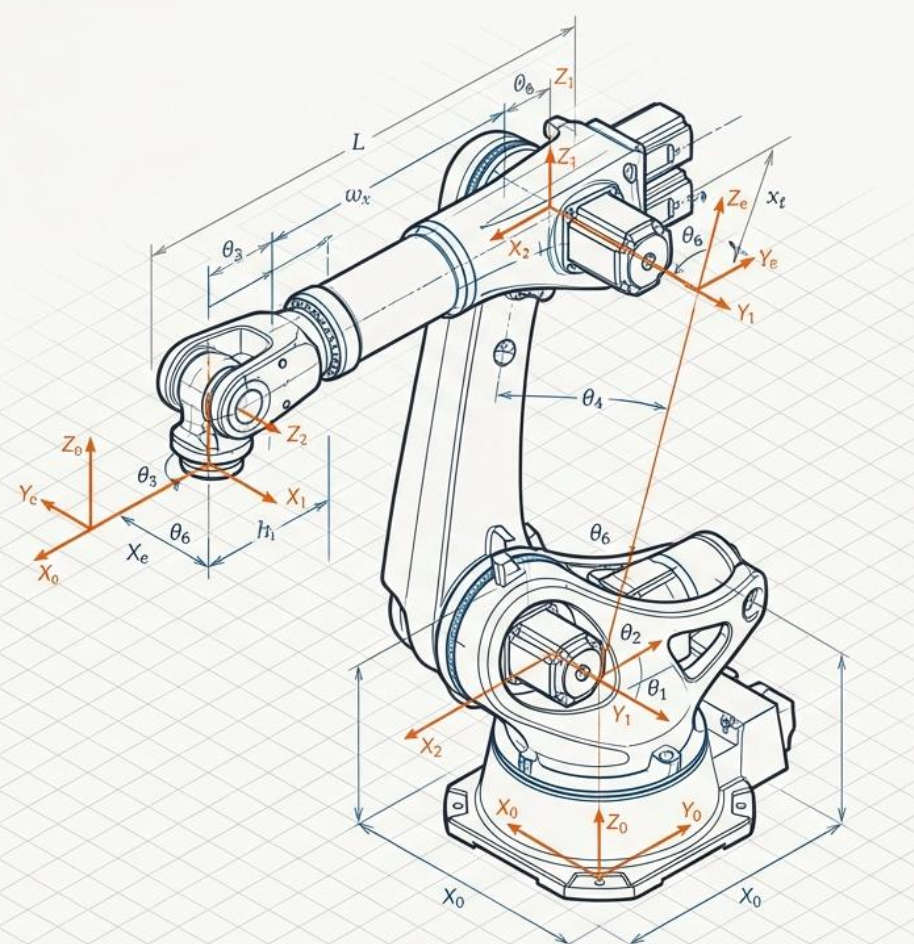
\includegraphics[width=0.5\linewidth]{assets/kin2.png}
    \caption{}\label{fig:}
\end{figure}
%
\section{Anatomia di una ``Serial Chain''}
Una Serial Chain è una sequenza di bracci che collegano la base all'end-effector, è composta da:
\begin{itemize}
    \item \emph{Link} (Bracci): Le parti rigide del corpo del robot;
    \item \emph{Joints} (Giunti): Connessioni che permettono il movimento relativo controllato (Rotoide, Prismatico, Sferico);
    \item \emph{Base}: Struttura connessa al suolo e al sistema di coordinate fisso del mondo;
    \item \emph{End-Effector}: Lo strumento funzionale finale che interagisce con l'ambiente.
\end{itemize}
\begin{figure}
    \centering
    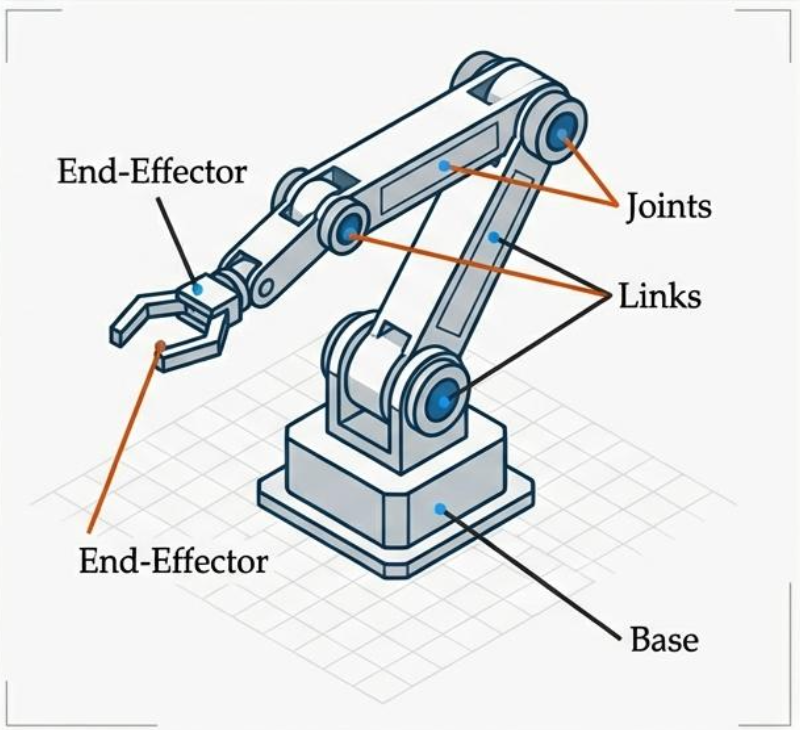
\includegraphics[width=0.5\linewidth]{assets/kinematics1.png}
    \caption{Anatomy of a serial chain}\label{fig:serialchain}
\end{figure}
%
\paragraph{Open Serial Chain} È una sequenza di bracci che collegano la base all'end-effector senza formare cicli chiusi.

%
\section{Degrees of Freedom e Orientamento nello spazio 3D}
I DoF sono il numero di parametri indipendenti necessari per definire completamente la configurazione di un meccanismo. In robotica, ogni DoF è solitamente associato a una specifica variabile di giunto:
\begin{itemize}
    \item \textbf{1 DOF}: Movimento vincolato lungo un singolo percorso (es. un treno su un binario);
    \item \textbf{2 DOF}: Movimento planare tramite due giunti indipendenti (traslazione in X e Y);
    \item \textbf{6 DOF}: Movimento non vincolato nello spazio 3D (3 traslazioni e 3 rotazioni).
\end{itemize}
%
\subsection{Il Problema dell'Orientamento nello Spazio 3D}
Tracciare un corpo rigido nello spazio è richiesto esprimere le coordinate di un \emph{frame relativo} alle coordinate di un \emph{frame rigido}.

\begin{theorem}[Position]
    La posizione di un corpo rigido è rappresentata da un vettore di traslazione $ 3 \times 1 $ ($ px, \, py, \, pz $).
\end{theorem}

\begin{theorem}[Orientation]
    L'orientamento è rappresentato da una matrice di rotazione $ R $ di dimensioni $ 3 \times 3 $.
\end{theorem}

\begin{remark}
    Ricordiamo infine che la posa (\emph{pose}) è data da:
    \[
        \text{Pose} = \text{Position} + \text{Orientation}
    \]
\end{remark}
\begin{figure}
    \centering
    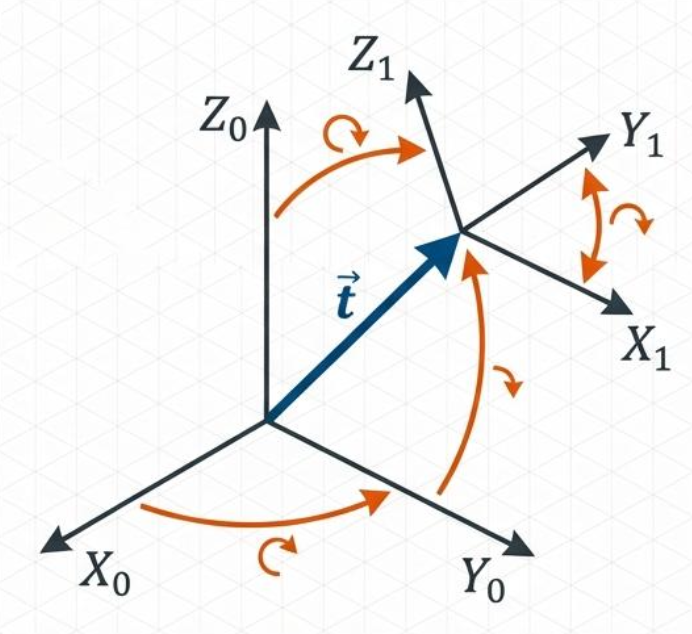
\includegraphics[width=0.5\linewidth]{assets/kin3.png}
    \caption{The Challenge of a 3D Space}\label{fig:kin3}
\end{figure}

%
\subsubsection{Descrivere l'Orientamento: gli Angoli di Eulero}
Gli angoli di Eulero (\textbf{Roll-Pitch-Yaw}, \textbf{Z-Y-X}) sono una rappresentazione minima dell'orientamento basata su 3 parametri indipendenti (3 rotazioni elementari in sequenza).

Questa rappresentazione fallisce quando la prima e l'ultima rotazione si allineano sullo stesso asse (ad esempio quando il \textbf{Pitch} raggiunge $\pm90^{\circ}$). Questo fenomeno causa la perdita di un grado di libertà ed è noto come \textbf{Gimbal Lock} (blocco cardanico).
\begin{theorem}[Singularity Condition]
    La condizione di singolarità negli angoli di Eulero è:
    \[
        \beta = \pm90^{\circ}
    \]
    Ne consegue la perdità di un DoF.
\end{theorem}
%
\section{Soluzione Unificata: Matrici Omogenee}
Le matrici omogenee $ 4 \times 4 $ rappresentano simultaneamente la rotazione ($3\times3$) e la traslazione ($3\times1$) all'interno di un'unica matrice.

Appartengono al gruppo speciale euclideo SE(3) e permettono di mappare i vettori da un sistema di riferimento all'altro senza singolarità:
\[
    \tilde{p}_{0} = A_{1}^{0}\tilde{p}_{1}
\]
Vedi figura \ref{fig:kin4}.
\begin{figure}
    \centering
    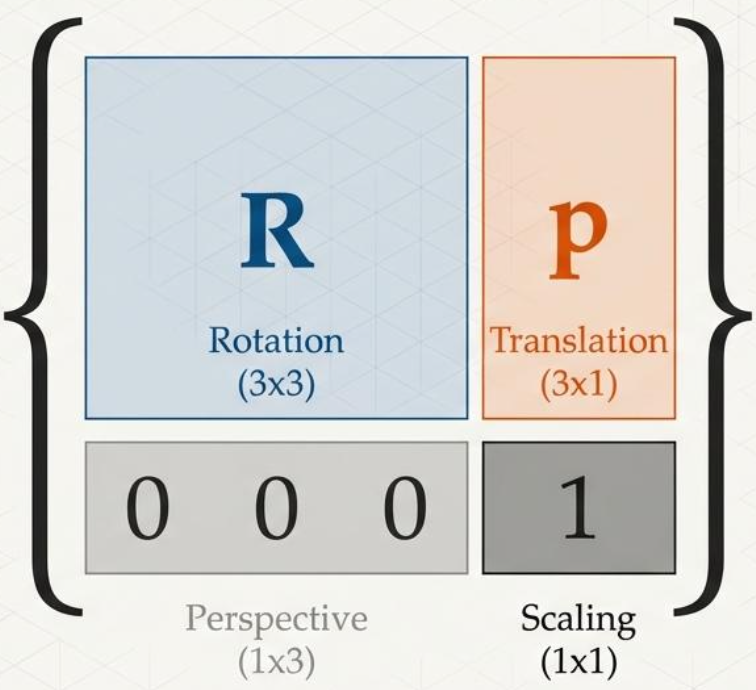
\includegraphics[width=0.5\linewidth]{assets/kin4.png}
    \caption{Homogeneous Matrices}\label{fig:kin4}
\end{figure}
%
\subsection{Composizione delle Trasformazioni}
Le matrici omogenee si moltiplicano in sequenza per calcolare i movimenti relativi lungo la catena seriale (\textbf{Chain Rule}):
\[
    {}^0T_n = {}^0T_1 \times {}^1T_2 \times \dots \times {}^{n-1}T_n
\]
Questo permette di mappare l'end-effector (${}^n$) direttamente rispetto alla base fissa (${}^0$) in un unico calcolo consolidato.

Vedi figura \ref{fig:kin5}.
\begin{figure}
    \centering
    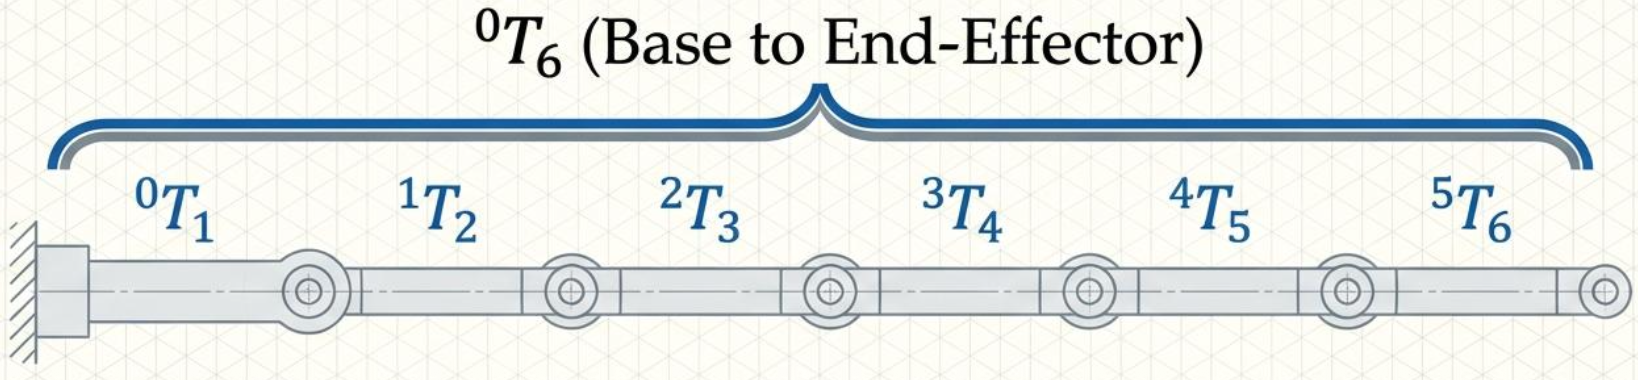
\includegraphics[width=\linewidth]{assets/kin5.png}
    \caption{Chain Rule}\label{fig:kin5}
\end{figure}

%
\subsection{Convenzione di Denavit-Hartenberg}
L'assegnazione arbitraria dei sistemi di riferimento richiede 6 parametri per link, risultando inefficiente. La convenzione \emph{D-H} è un sistema sistematico che riduce i requisiti a esattamente 4 parametri per link:
\begin{enumerate}
    \item  $ a_{i} $ (Link Length): Traslazione lungo l'asse $x$.
    \item $\alpha_i$ (Link Twist): Rotazione attorno all'asse $x$.
    \item $d_i$ (Joint Offset): Traslazione lungo l'asse $z$ (è la variabile nei giunti prismatici).
    \item $\theta_i$ (Joint Angle): Rotazione attorno dell'asse $z$ (è la variabile nei giunti rotoidi).
\end{enumerate}
Vedi figura \ref{fig:kin6}.
\begin{figure}
    \centering
    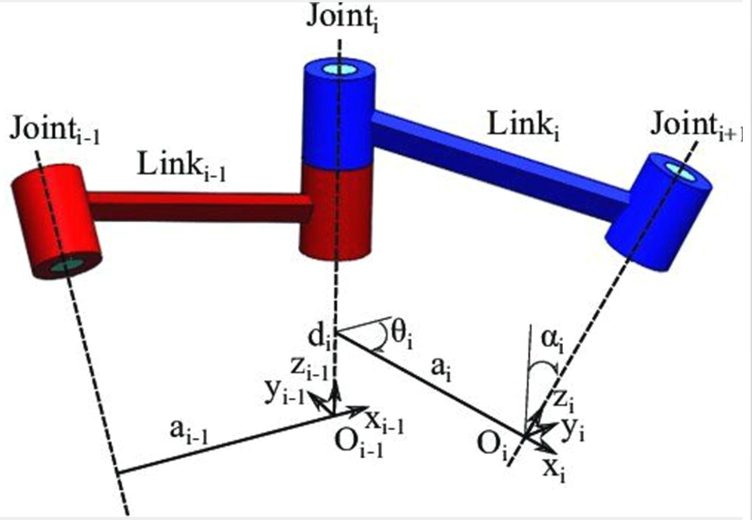
\includegraphics[width=0.7\linewidth]{assets/kin6.png}
    \caption{4 Parametri della convenzione D-H}\label{fig:kin6}
\end{figure}
%
\begin{theorem}[D-H Matrix]
    È la matrice di trasformazione omogenea generale per un singolo giunto utilizzando i parametri D-H:
    \[
        A_i^{i-1} = \begin{bmatrix}
            \cos\theta_i & -\sin\theta_i\cos\alpha_i & \sin\theta_i\sin\alpha_i  & a_i\cos\theta_i \\
            \sin\theta_i & \cos\theta_i\cos\alpha_i  & -\cos\theta_i\sin\alpha_i & a_i\sin\theta_i \\
            0            & \sin\alpha_i              & \cos\alpha_i              & d_i             \\
            0            & 0                         & 0                         & 1
        \end{bmatrix}
    \]
    Questa matrice finale è funzione di una sola variabile di giunto ($q_i$) e viene generata dal prodotto di quattro trasformazioni di base:
    \[
        \text{Rot}(z,\theta) \times \text{Trans}(z,d) \times \text{Trans}(x,a) \times \text{Rot} (x,\alpha)
    \]
\end{theorem}
\section{I Due Problemi Fondamentali della Cinematica}

La cinematica analizza la geometria del movimento tridimensionale traducendo le relazioni tra lo spazio dei giunti e lo spazio operativo dell'end-effector[cite: 388, 390]. Si divide in due problemi speculari[cite: 544]:

\subsection{Cinematica Diretta (Forward Kinematics)}

Rappresenta il problema computazionalmente ``facile'' della cinematica spaziale[cite: 564].

\begin{description}
    \item[Definizione:] Determinare la posizione e l'orientamento dell'end-effector conoscendo la configurazione dei giunti[cite: 548].
    \item[Input:] Variabili di giunto (rotazioni $\theta$, traslazioni $d$) e lunghezze stabili dei bracci[cite: 565, 566].
    \item[Output:] Posa cartesiana esatta (posizione ed orientamento) dell'end-effector nello spazio[cite: 568].
    \item[Formulazione Matematica:] Il calcolo si esegue interamente tramite la moltiplicazione sequenziale delle matrici di trasformazione dei singoli giunti (regola della catena)[cite: 573]:
          \begin{equation}
              x_n = A_{n-1}A_{n-2}\dots A_1A_0x_0
          \end{equation}
          Espresso in forma sintetica attraverso il prodotto delle matrici omogenee[cite: 475]:
          \begin{equation}
              {}^0T_n = {}^0T_1 \times {}^1T_2 \times \dots \times {}^{n-1}T_n
          \end{equation}
    \item[Soluzioni:] Produce sempre \textbf{un'unica soluzione univoca e garantita}[cite: 575].
\end{description}

\subsection{Cinematica Inversa (Inverse Kinematics)}

Rappresenta il problema matematicamente ``difficile'' della cinematica robotica[cite: 579].

\begin{description}
    \item[Definizione:] Calcolare la configurazione che i giunti devono assumere per posizionare lo strumento secondo una posa cartesiana desiderata[cite: 551].
    \item[Input:] Posa cartesiana tridimensionale desiderata per l'end-effector[cite: 580].
    \item[Output:] Angoli di rotazione o estensioni lineari dei singoli giunti richiesti[cite: 581].
    \item[Calcolo Matematico:] Richiede l'inversione di matrici geometriche complesse e la risoluzione di \textbf{equazioni algebriche fortemente non lineari} (presenza di seni e coseni accoppiati)[cite: 582].
    \item[Analisi delle Soluzioni:] A causa della non linearità, l'inversione può determinare tre scenari fisici differenti[cite: 583, 584]:
          \begin{itemize}
              \item \textbf{Soluzioni multiple:} Lo stesso punto nello spazio operativo è raggiungibile attraverso diverse configurazioni geometriche del braccio.
              \item \textbf{Infinite soluzioni:} Si verifica in presenza di robot cinematicamente ridondanti (gradi di libertà superiori a quelli richiesti).
              \item \textbf{Zero soluzioni:} Il target richiesto si trova all'esterno dell'inviluppo di lavoro raggiungibile dal robot (oltre il workspace limit).
          \end{itemize}
\end{description}

\section{La Pipeline Robotica}
La cinematica fornisce lo schema fondamentale delle capacità spaziali del robot e si inserisce in una struttura di controllo software a livelli:
\begin{enumerate}
    \item \textbf{Task Planning} (Posa desiderata): Definizione degli obiettivi ad alto livello, generazione delle traiettorie ed evitamento degli ostacoli.
    \item \textbf{Cinematica Inversa} (Angoli di giunto): Mappatura della posa finale nelle configurazioni di giunto richieste. Serve anche da fondamento per la cinematica differenziale inversa (Jacobiani/Velocità).
    \item \textbf{Dinamica} (Coppie e Forze): Calcolo delle forze e delle coppie fisiche necessarie ai motori basandosi su massa, inerzia e movimento.
    \item \textbf{Robot Controller} (Comandi del motore): Esecuzione in tempo reale, driver dei motori e cicli di feedback.
\end{enumerate}